

%interpretation of results
\section{Interpretation of Results}
%interpreting EKF results
\subsection{EKF likelihood}
 In section~\ref{sec: EKF test} I found that the likelihood obtained using the EKF performs slightly worse than the EM method for the parameters $\beta_1$ and $\beta_2$. A reason for this might be that the method was tested in a scenario where the Brownian motion is much larger than the drift in the Langevin process, which is what one might expect in an animal setting. This makes the predict steps of the EKF undershoot the steps of the Langevin process. In turn, this leads to an error, which is compounded every time the predict step is performed. If the position used in the predict step is wrong, the prediction of the covariance using the curvature of the covariates also becomes wrong. To see how the EKF works in practice, I used the covariates from earlier and plotted the predict steps of the Langevin process together with steps of the EKF, and the 90\% confidence level using the predicted covariance. The results are shown in figure~\ref{fig:EKF high diffusion}. 


\begin{figure}[H]
    \centering
    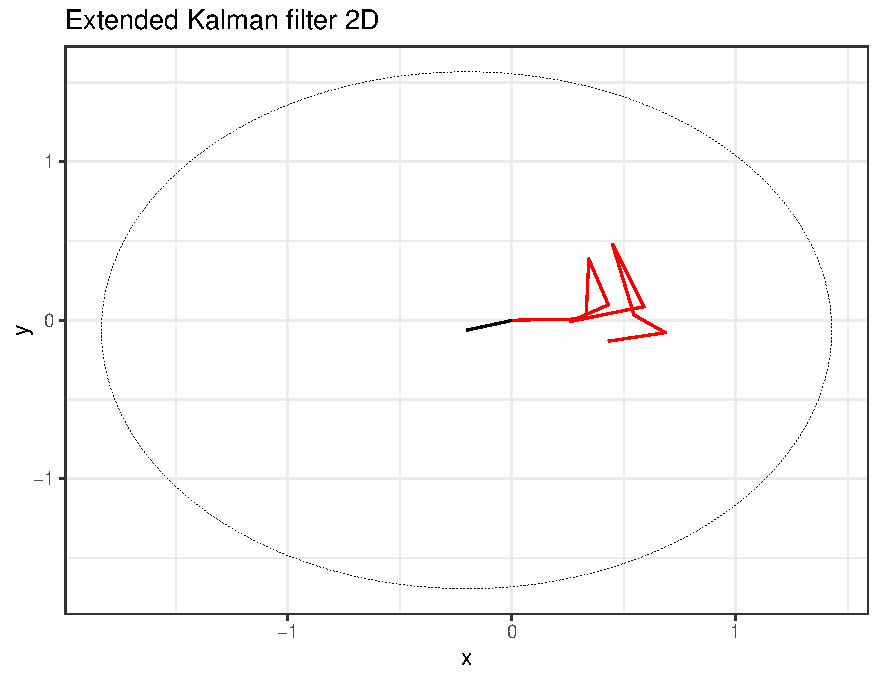
\includegraphics[width=\linewidth]{Images/discussion/EKF high diffusion path.pdf}
    \caption[EKF path]{The black line shows state estimates of the Langevin process using the predict step of the EKF. The red line shows a Langevin track that we are estimating, simulated at a resolution of $0.01$ using 10 steps. The dotted ellipse shows the 90\% confidence level set of the final predicted state. The parameters used are the same for the Langevin process and the EKF.}
    \label{fig:EKF high diffusion}
\end{figure}

The code for generating Figure~\ref{fig:EKF high diffusion} can be found in the github repository in Appendix~\ref{Appendix: github repo} under the file name "EKF path figure.R". Figure~\ref{fig:EKF high diffusion} shows that there is little correspondence between the path of the predictions made by the EKF and the Langevin process. In this case, the paths have ended up going in almost opposite directions. This happens because the Langevin process pictured is dominated by randomness, which also means that the Langevin path is much longer than the path from the EKF. Since the intermediate values of EKF do not approximate the intermediate values of the Langevin process wee, doing multiple steps of the EKF might not make an improvement to the estimate.
The EKF might work better. Using intermediate predict steps in the EKF might work better in scenarios where the diffusion is smaller and the drift larger, since the predictions would deviate less from the true values of the Langevin process.



%interpreting results from scenario 1
\subsection{Scenario 1}
\label{subsec: Scenario 1 interpretation}
In Scenario 1 in Section~\ref{sec: BB test} we saw that the method using the Brownian bridge importance sampling likelihood eliminated the bias observed in the estimates using the EM method in figure~\ref{fig:EM_thin_boxplot}. This is not surprising because the importance sampling estimate should converge to the correct value of the likelihood and because the proposal being used is similar to the Langevin process. The test also showed that there were two estimates that overestimated the value of the parameter $\gamma^2$ by a large margin. This might be due to the method that was used to find the maximum likelihood estimate. The maximum likelihood was found by using the "L-BFGS-B" method implemented in the R-package "optim", and the likelihood function simulated new Brownian bridges each time it was evaluated. This meant that the likelihood was stochastic, which could mean that the optimization algorithm found a value of the likelihood that had a high value due to randomness. The estimates that were found were still an improvement on the estimates using the EM method, but they could perhaps be further improved by simulating standard Gaussian variables $\textbf{Z}$ beforehand, then transforming them by using $\gamma \textbf{Z} +\mu$ to give Brownian bridges scaled with the right speed parameter. The likelihood estimates obtained by doing this would be deterministic, which might reduce the variance of the estimates and hinder outliers.



Another observation from Scenario 1 is that the variance of the $\bm \beta$-parameters is reduced as the time difference of the observations increases, when the number of observations is held constant. This was observed both when the Brownian bridges were, and were not precomputed. The same explanation as was used to explain the same phenomenon for the EM estimates can be used in this case: that when more of the covariate range is explored, the variance of the coefficient estimates is reduced. Since estimates are unbiased at all values of $dt$, this suggests that if we are given the choice between a higher frequency of observations of an animal's movement or a lower frequency, we should prefer the lower frequency, given that they have the same cost to acquire.


In Scenario 1 in Section~\ref{sec: BB test} we saw that the estimator using the precomputed Brownian bridge importance sampling likelihood is an improvement over the EM estimates for all parameters. At a thinning of 10 there is little or no bias in the estimates, whereas using the EM method, there is an observable bias at this value of $\Delta_t$. For the speed parameter $\gamma^2$, we see that there is a bias observed for thinning of 50 and 100. In both of these cases, all the estimations performed significantly underestimated the value of the parameter. One reason for this must be that the Brownian bridges become a much worse proposal density when the speed parameter used for generating the Brownian bridges deviates from the parameter which is being used to compute the likelihood. 
When $\Delta_t=0.1$ there is bias in the EM method whose $\gamma^2$ estimates are used to simulate Brownian bridges, however, there is no bias seen in figure~\ref{fig:varying dt boxplot precomputed BB} for this value of $\Delta_t$. This suggests that even if the value used to generate the bridges is slightly off, the likelihood can still be accurately approximated using this proposal, but for larger discrepancies, the method breaks down. 



A striking feature of the estimations done using precomputed Brownian bridges is that even though there is a large bias in the speed parameter $\gamma^2$, there appears to be little or no bias in the estimates of $\bm \beta$. This is particularly interesting, since the drift term in the Langevin process is scaled by $\gamma^2$. This might suggest that the variance used to make the Brownian bridges is not important when it comes to estimating $\bm \beta$, but is more important when it comes to estimating $\gamma^2$. 




%interpretation of scenario 2
\subsection{Scenario 2}
\label{subsec: scenario 2 interpretation}

In the simulations done in scenario 2 we saw that both when using and not using precomputed Brownian bridges, there is a bias in the estimates of $\beta_1$ and $\beta_2$ when the number of nodes in the bridges becomes small. Interestingly, this is the opposite of the bias seen in the EM estimates. As the number of nodes in the bridges decreases, one would think that the importance sampling estimates should approach that of the EM estimates, since we would get the same error with the discretization. It is difficult to say exactly why this is not observed. For the $\gamma^2$ estimate when not using precomputed bridges, we observe what we would expect from the EM method: that there is a bias toward zero.




%interpretation of scenario 3
\subsection{Scenario 3}
\label{subsec: scenario 3 interpretation}


When not using precomputed bridges, we saw in Scenario 3  that for small M, there was a bias in the estimates. One reason for this might be that the number of bridge nodes $N$ used was less than the number of steps used to simulate the data. However, as $M$ increased, this bias disappeared. This can be explained by the fact that even if we are using a nonoptimal proposal density, the importance sampling estimate should still converge to the correct likelihood as $M$ increases. It also suggests that even if the number of bridge nodes $N$ is not enough to simulate the Langevin process, if we have enough of these bridges, we can still get unbiased estimates. Another observation from Scenario 3 is that the variance of the estimates decreases as $M$ increases. This makes sense since when we are using more bridges, we are averaging over more paths to find the likelihood.


%precomputed
When using precomputed bridges, the same pattern was seen. For a small number of bridges, there were large biases for $\beta_1$, $\beta_2$, and $\gamma^2$. However, as $M$ increased, the biases seen in $\beta_1$ and $\beta_2$ were eliminated, and the bias seen in $\gamma^2$. For all values of $M$ tried, there was a bias in $\gamma^2$, but it is reasonable to think that if $M$ becomes large enough, the bias seen in $\gamma^2$ when using precomputed Brownian bridges will disappear. This might mean that precomputing the bridges might still be the better method if it can make up for the fact that more bridges are simulated by the fact that it is faster.


\subsection{Computation Time}

In Subsection~\ref{subsec: computation time} we found that for the given scenario, the average computation time using precomputed Brownian bridges was 9.90 minutes and when not using precomputed bridges it was 18.89 minutes. This means that there was some efficiency to be gained from precomputing the Brownian bridges. However, since using precomputed Brownian bridges gives the wrong estimates, this method should not be preferred over the alternative. As was discussed in Scenario 3, the method using precomputed Brownian bridges might give unbiased estimates if the number of bridges used is sufficiently high, and the efficiency gain of precomputing the bridges might make up for the fact that more bridges have to be computed.


The standard deviation of the computation time when using precomputed Brownian bridges was 0.50 minutes, and when not using precomputed bridges it was 4.49 minutes. One explanation for the larger deviation in computation time when not precomputing the bridges might be that the likelihood in this case is stochastic. This might make the optimization algorithm find a point that by chance has a high value, which would make it stop early. Because of this, as mentioned earlier, simulating standard Brownian bridges, then scaling them when computing the likelihood, might be better for likelihood maximization.





\section{Limitations and Future Directions}
The method using Brownian bridge importance sampling showed promising results when it comes to eliminating the bias seen in the EM method. However, a problem with using this method is that it cannot handle observation errors. Typically, track data is collected with some observation error, for example from getting positions by GPS. If this error is not taken into account, the estimates would no longer be accurate. \textcite{michelot_langevin_2019} circumvents this problem by using the Kalman filter to find predicted positions that are then used to estimate the parameters. Another possibility is that, when the distance between observations becomes large, the effect of the observation error on parameter estimates becomes less significant. However, this is something that would need to be studied further. Alternatively, Appendix~\ref{Appendix: Langevin with obs error} contains a derivation of a likelihood estimator for the Langevin process with normally distributed observation error. I have not made this estimator work in practice, so it is not in the main section of this thesis.



In addition to this, the gradient used to optimize the sampling likelihood of Brownian bridge importance sampling likelihood was approximated by not taking the derivative by treating the bridges if they were not dependent on $\gamma^2$. Alternatively, the gradient can be approximate numerically, which would require the Brownian bridges to be scaled instead of re-simulated. In this thesis, no tests were done to see if a numerical approximation of the gradient would give a different result to the likelihood maximization.


In this thesis, I have not explored how to choose the number of bridge nodes $N$ or the number of bridges $M$ that should be used in the Brownian bridge importance sampling likelihood to eliminate the bias and reduce the variance of the estimator. If the number of bridge nodes $N$ is low, the estimates become biased; however, this can be compensated for by using more bridges. To see that the values of $N$ and $M$ are large enough, multiple values should be tried when fitting the model. If $M$ and $N$ are large enough, there should be small changes in the estimate when their values are increased. 


The Langevin movement model is a simple model that cannot model more complex animal behaviors. For example, some animal might show directional persistence in their movement. That is, they tend to move in the same direction as they are already traveling. This is in contrast to the Langevin movement model, in which any direction is equally likely to travel. Another behavior that one might think an animal might show is that the areas they occupy might change over time. To model this would require time-varying covariates, which is not something that can be done using the Langevin movement model. However, the model can include a time-varying speed parameter $\gamma^2$\parencite{michelot_langevin_2019}.


Another topic that was not explored in this thesis is which proposal to use in importance sampling. In addition to using Brownian bridges as a proposal, \textcite{durham_numerical_2002} also uses what they call a "modified Brownian bridge" that has a variance that decreases as the bridge goes from the start to the end point. They show that this gives a lower mean square error when approximating the Langevin likelihood. There might also be other improvements that can be made, like using other forms of interpolation than linear interpolation for the mean of the bridges. These improvements could possibly make the method more efficient and reduce computation time.

